%!TEX root =  ../main.tex
\renewcommand{\columnseprule}{1.5pt}
\begin{multicols*}{2}
\rule[0.5\baselineskip]{0.4\textwidth}{1pt}
\noindent
\LabSection{``Upside Down''}\label{sec:0404p}
\begin{exercises}{sec:0404p}
\lab{} We want to be able to transform any graph into its reciprocal.  Graph $y=x$ and $y=4/x$, either in different colors or in different line styles below.

\noindent
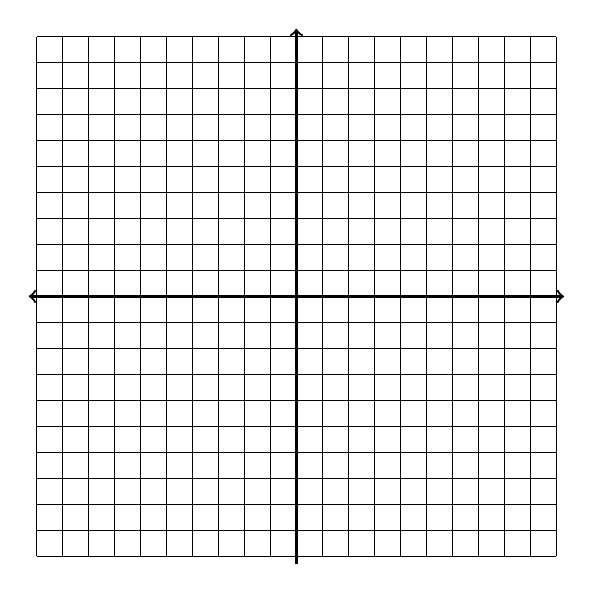
\begin{tikzpicture}[xscale=0.33,yscale=0.33]
	\draw [thick, <->] (-10.3,0) -- (10.3,0);
	\draw [thick, ->] (0,-10.3) -- (0,10.3);
	\draw [thin] (-10,-10) grid (10,10);
\end{tikzpicture}

\lab{} What points are in common between the two graphs?  How is this the same question as “What numbers are their own reciprocals?”

\vspace{3cm}
\lab{} What number is the reciprocal of 2?  Find the \emph{eight} points that illustrate that fact.


\vspace{4cm}
\lab{}  What number is the reciprocal of 0?  Why is this a trick question?  What behavior do graphs exhibit close to a ``divide by 0''?

\vspace{3cm}
\lab{} Construct a set of rules to help you graph reciprocals.  What happens to positives and negatives?  1s?  2s?  0s?


\vspace{4cm}
\lab{} Graph $f(x)=x^2-6x+5$ and its reciprocal by hand

\noindent
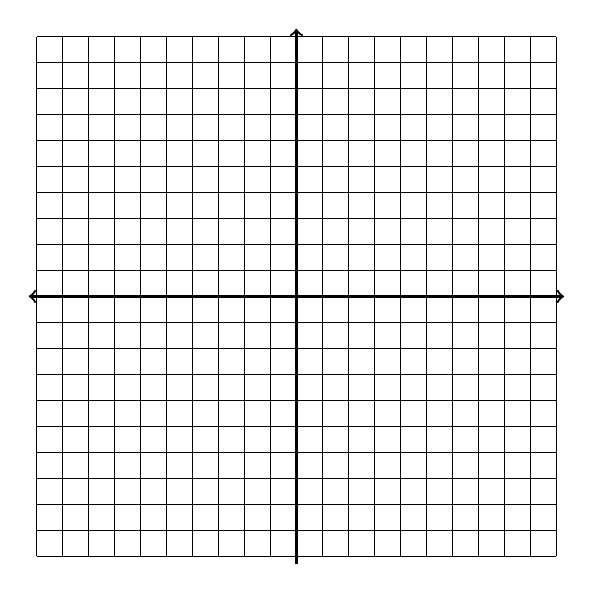
\begin{tikzpicture}[xscale=0.33,yscale=0.33]
	\draw [thick, <->] (-10.3,0) -- (10.3,0);
	\draw [thick, ->] (0,-10.3) -- (0,10.3);
	\draw [thin] (-10,-10) grid (10,10);
\end{tikzpicture}

\lab{} Describe a hypothetical situation where someone might graph one ratio on accident, and actually want the reciprocal.


\end{exercises}
\end{multicols*}